\documentclass[a4paper,12pt]{article}
\usepackage[T1,T2A]{fontenc}
\usepackage[utf8]{inputenc}
\usepackage[english,ukrainian]{babel}


\usepackage{ upgreek }
\usepackage{amsmath}

\usepackage{graphicx}
\graphicspath{{./pictures/}}


\usepackage[unicode=true,colorlinks=true,urlcolor=blue,citecolor=green,linkcolor=blue]{hyperref}
\usepackage[ukrainian,nameinlink]{cleveref}
\usepackage{geometry} % Меняем поля страницы
\geometry{left=2cm}% левое поле
\geometry{right=1.5cm}% правое поле
\geometry{top=1cm}% верхнее поле
\geometry{bottom=2cm}% нижнее поле



\begin{document}
	
	\begin{titlepage}
		\vspace*{6cm}
		\begin{center}
			
			\large
			\textbf{Звіт}\\
			\textbf{до лабораторної роботи №6:}\\
			\textbf{<<Перевірка гіпотези про однорідність вибірок за допомогою статистики Петуніна>>}
			
		\end{center}
		
		\vspace{8cm}
		\begin{flushright}
			студента 1-го курсу магістратури\\
			факультету комп'ютерних наук та кібернетики\\
			Кравця Олексія
		\end{flushright}
		
	\end{titlepage}

\newpage
\tableofcontents
\newpage
%document here

\section{Теоретичні відомості}

\textbf{Статистика Петуніна }(p-статистика) — міра близькості між вибірками, запропонована українським математиком Юрій Петуніним. Використовується для перевірки гіпотези про рівність функцій розподілу двох вибірок.

Розглянемо дві генеральні сукупності $G$, $G'$ та відповідні функції розподілу $F_G$, $F_{G'}$. 

Нехай задано дві вибірки $x = (x_1, x_2 , \ldots, x_n) \in G$ та $x' = (x_1', x_2', \ldots, x_m') \in G'$, а $x_{(1)} \le x_{(2)} \le \ldots \le x_{(n)}$ та $x_{(1)}' \le x_{(2)}' \le \ldots \le x_{(m)}'$ -- відповідні порядкові статистики  та необхідно визначити, чи вони належать однаковим розподілам. Припустимо, що $F_G(u) = F_{G'}(u)$, тоді

\[
	P(A_{ij}) = P \left(x_k' \in (x_{(i)}, x_{(j)}) \right) = p_{ij} = \frac{j-i}{n+1}
\]

Якщо маємо вибірку $x' \in (x_{(1)}', x_{(2)}', \ldots, x_{(m)}' )$, можемо знайти частоту $h_{ij}$ випадкової події $A_{ij}$ та довірчі інтервали $(p_{ij}^{(1)},p_{ij}^{(2)})$ для ймовірності $p_{ij}$ при заданому рівні значущості $\beta$, тобто $B = \left\{ p_{ij} \in (p_{ij}^{(1)},p_{ij}^{(2)})\right\}$, $P(B) = 1 - \beta$. Тоді

\[
	p_{ij}^{(1)} = \frac{h_{ij}m + \frac{g^2}{2} - g \sqrt{h_{ij}(1 - h_{ij})m + \frac{g^2}{4}}}{m + g^2}
\]

\[
	p_{ij}^{(2)} = \frac{h_{ij}m + \frac{g^2}{2} + g \sqrt{h_{ij}(1 - h_{ij})m + \frac{g^2}{4}}}{m + g^2}
\]

де $g$ задовольняє умову $\phi(g) = 1 - \frac{\beta}{2}$ ($\phi(g)$ -- щільність нормального розподілу).Покладемо $g =3$. Величина $g$ визначає рівень значущості довірчого інтервалу  $I^{(n,m)}_{ij} = (p_{ij}^{(1)},p_{ij}^{(2)})$. В силу правила $3 \sigma$ рівень значущості цього інтервалу не перевищує $0.05$. 

Позначимо через $N$ кількість довірчих інтервалів $I_{i,j} = (p_{ij}^{(1)},p_{ij}^{(2)})$, також $N = \frac{n(n-1)}{2}$. Позначимо $L$ -- кількість тих інтервалів $I_{ij}$, які містять ймовірність $p_{ij}^{(n)}$. Статистику $h_{ij} = \frac{L}{N}$ будемо називати $p$-статистикою і вона буде мірою близькості $\rho(x,x')$ між вибірками $x$, $x'$.


\section{Практичні результати}

Для тестування візьмемо вибірку з нормального розподілу $N(0,1)$, розмір вибірки $m = 200$ елементів. 

Перевіримо гіпотезу про рівність функцій розподілу для нормальних розподілів $N(\mu, 1)$, де $\mu$ змінюється від $-2$ до $2$ з кроком $0.1$. Розмір кожної вибірки $n =100$. Отримаємо рисунок \ref{fig:f1}. Бачимо на осі абсцис значення $\mu$ на осі ординат значення $p$-статистики.

\newpage
\begin{figure}[ht]
	\center{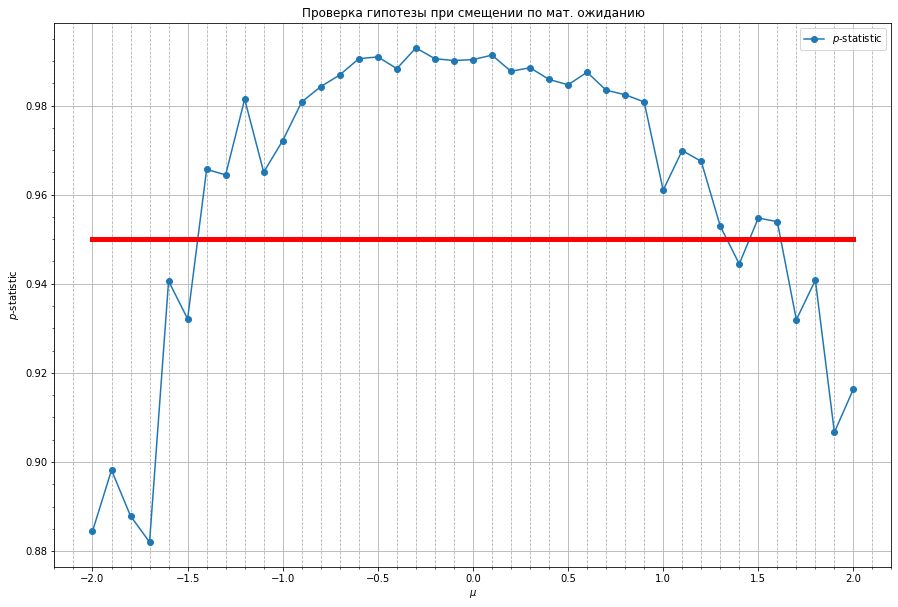
\includegraphics[scale=0.5]{fig1.png}}
	\caption{Перевірка гіпотези при зміщенні по мат. сподіванню}
	\label{fig:f1}
\end{figure}

Гіпотезу \textbf{не відхиляємо} при наступних значеннях $\mu$:
\begin{verbatim}
	array([-1.4, -1.3, -1.2, -1.1, -1. , -0.9, -0.8, -0.7, -0.6, -0.5, -0.4,
	-0.3, -0.2, -0.1,  0. ,  0.1,  0.2,  0.3,  0.4,  0.5,  0.6,  0.7,
	0.8,  0.9,  1. ,  1.1,  1.2,  1.3,  1.5,  1.6])
\end{verbatim}

Перевіримо гіпотезу про рівність функцій розподілу для нормальних розподілів $N(0, \sigma)$, де $\sigma$ змінюється від $0.1$ до $3$ з кроком $0.1$. Розмір кожної вибірки $n =100$. Отримаємо рисунок \ref{fig:f2}. Бачимо на осі абсцис значення $\mu$ на осі ординат значення $p$-статистики

\newpage
\begin{figure}[ht]
	\center{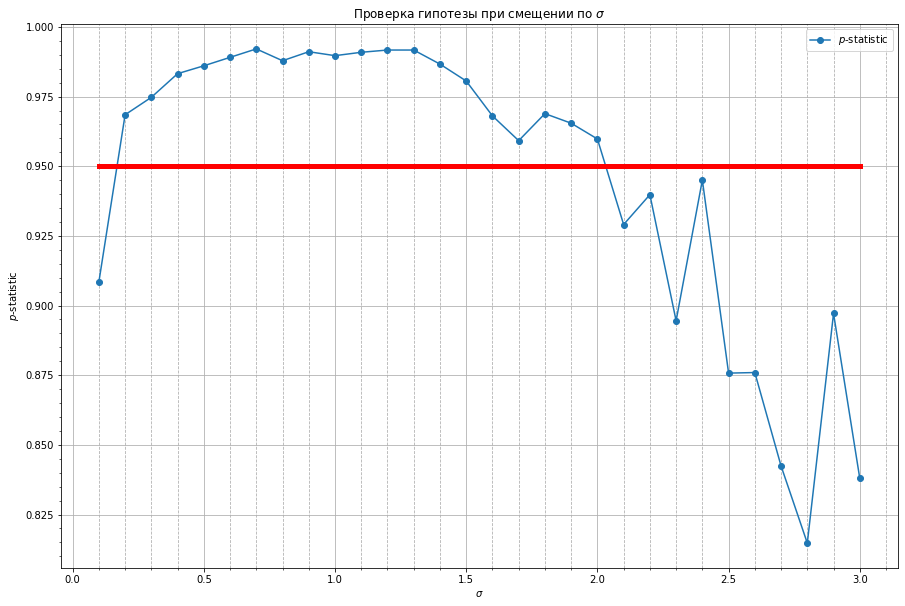
\includegraphics[scale=0.5]{fig2.png}}
	\caption{Перевірка гіпотези при зміщенні $\sigma$}
	\label{fig:f2}
\end{figure}

Гіпотезу \textbf{не відхиляємо} при наступних значеннях $\sigma$:
\begin{verbatim}
	array([0.2, 0.3, 0.4, 0.5, 0.6, 0.7, 0.8, 0.9, 1. , 1.1, 1.2, 1.3, 1.4,
	1.5, 1.6, 1.7, 1.8, 1.9, 2. ])
\end{verbatim}

\addcontentsline{toc}{section}{Література}
\begin{thebibliography}{}
	\bibitem{wiki} \href{https://uk.wikipedia.org/wiki/%D0%A1%D1%82%D0%B0%D1%82%D0%B8%D1%81%D1%82%D0%B8%D0%BA%D0%B0_%D0%9F%D0%B5%D1%82%D1%83%D0%BD%D1%96%D0%BD%D0%B0}{https://uk.wikipedia.org/wiki/Статистика\_Петуніна}
	\bibitem{lection} \href{http://om.univ.kiev.ua/users_upload/15/upload/file/pr_lecture_13.pdf}{Лекція 13. Непараметрична класифікація за допомогою р-статистики, Клюшин Дмитро Анатолійович}
\end{thebibliography}

\end{document}
